% --- ETUDE DE CAS ---
\newpage

\section*{AAV}
\addcontentsline{toc}{section}{AAV}
\begin{itemize}
	\item [6] Développer des composants réutilisables
	\item [3] Employer un access store
	\item [5] Interagir avec les composants (hooks)
	\item [5] Utiliser (Modéliser) JWT pour le processus d'authentification
	\item [4] Utiliser le système de loadbalancing pour réaliser le routage
\end{itemize}

\newpage

\section*{Étude de cas~: Sécurité}
\addcontentsline{toc}{section}{Étude de cas~: Sécurité}

\subsection*{Mots clés}
\phantomsection
\addcontentsline{toc}{subsection}{Mots clés}
\begin{itemize}
	\item CORS
	\item React context
	\item Provider
	\item Access store
	\item Hooks
	\item Loadbalancing
\end{itemize}

\subsection*{Contexte}
\phantomsection
\addcontentsline{toc}{subsection}{Contexte}
\noindent Yanis a fini de dev la partie token de son backend, cependant un problème persiste. Il se pose donc des questions sur la sécurité frontend de son site web.

\subsection*{Problématique}
\phantomsection
\addcontentsline{toc}{subsection}{Problématique}
\noindent Comment sécuriser son token coté frontend ?

\subsection*{Contraintes}
\phantomsection
\addcontentsline{toc}{subsection}{Contraintes}
\begin{itemize}
	\item JWT
	\item React
	\item Problèmes de CORS
\end{itemize}

\subsection*{Généralisation}
\phantomsection
\addcontentsline{toc}{subsection}{Généralisation}
\begin{itemize}
	\item Sécurité
	\item Gestion des secrets
\end{itemize}

\subsection*{Livrables}
\phantomsection
\addcontentsline{toc}{subsection}{Livrables}
\begin{itemize}
	\item Code frontend sécurisé avec le token caché
\end{itemize}

\newpage

\subsection*{Pistes de solutions}
\phantomsection
\addcontentsline{toc}{subsection}{Pistes de solutions}
\begin{itemize}
	\item React Context combinée à des hooks
	\item CORS
\end{itemize}

\subsection*{Plan d'actions}
\phantomsection
\addcontentsline{toc}{subsection}{Plan d'actions}
\begin{itemize}
	\item DMC / ER
	\item Étudier le fonctionnement du CORS
	\item Se renseigner sur les failles de sécurités actuel 
	\item Se renseigner sur les solutions actuel / les bonnes pratiques
	\item Sécuriser le frontend
\end{itemize}

\newpage

\section*{Définition~: Mots clés}
\phantomsection
\addcontentsline{toc}{section}{Définition~: Mots clés}

\subsubsection*{CORS}
\phantomsection
\addcontentsline{toc}{subsection}{CORS}

\noindent Le \textbf{CORS} (\textit{Cross-Origin Resource Sharing}, \og{}partage des ressources entre origines\fg{}) est un \textbf{mécanisme de sécurité du navigateur} qui contrôle si une page web servie par une \textbf{origine} (couple \textbf{protocole + domaine + port}) a le droit d'appeler une API hébergée sur une \textbf{origine différente}. Par défaut, la \textbf{politique du même origine} (\textit{Same-Origin Policy}) \textbf{bloque} ces requêtes croisées pour protéger l'utilisateur. Le serveur autorise explicitement le front-end en renvoyant des \textbf{en-têtes HTTP} dédiés~:
\begin{itemize}
	\item \texttt{Access-Control-Allow-Origin}~: l'origine (ex.~\texttt{https://app.breezy.fr}) autorisée à consommer l'API~;
	\item \texttt{Access-Control-Allow-Methods}~: les méthodes permises (\texttt{GET}, \texttt{POST}…)~;
	\item \texttt{Access-Control-Allow-Headers}~: les en-têtes acceptés, notamment \texttt{Authorization} qui porte le \textbf{JWT}.
\end{itemize}
\begin{center}
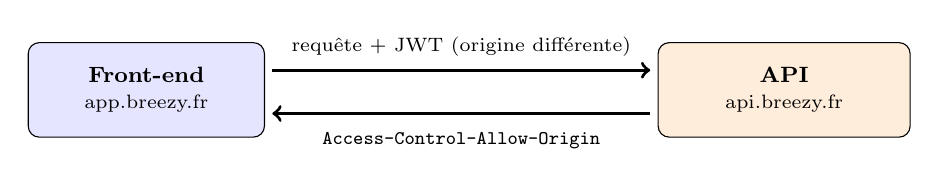
\begin{tikzpicture}[font=\footnotesize]
	\draw[fill=blue!10, rounded corners] (0,0.6) rectangle (3.0,1.8) node[midway, align=center]{\textbf{Front-end}\\\scriptsize app.breezy.fr};
	\draw[fill=orange!14, rounded corners] (8.0,0.6) rectangle (11.2,1.8) node[midway, align=center]{\textbf{API}\\\scriptsize api.breezy.fr};
	\draw[->, very thick] (3.1,1.45) -- (7.9,1.45); \node at (5.5,1.75){\scriptsize requête + JWT (origine différente)};
	\draw[<-, very thick] (3.1,0.9) -- (7.9,0.9); \node at (5.5,0.55){\scriptsize \texttt{Access-Control-Allow-Origin}};
\end{tikzpicture}
\end{center}
\noindent\textit{Figure~: sans en-tête CORS adéquat, le navigateur bloque l'appel inter-origines.} Dans le projet, le front-end React et l'API étant sur des origines distinctes, une \textbf{configuration CORS correcte} (côté serveur) est indispensable pour que le \textbf{JWT} puisse être transmis~; c'est l'une des contraintes explicites de l'étude de cas.

\vspace{0.4cm}

\subsubsection*{React Context}
\phantomsection
\addcontentsline{toc}{subsection}{React Context}

\noindent Le \textbf{React Context} est le mécanisme natif de React permettant de \textbf{partager une donnée} (utilisateur connecté, thème, \textbf{jeton JWT}) avec un \textbf{ensemble de composants} sans la faire transiter manuellement de parent en enfant via les props. Il résout le problème du \textbf{\og{}prop drilling\fg{}}~: faire descendre une même valeur à travers de nombreux niveaux intermédiaires qui n'en ont pas l'usage. Un contexte se crée avec \texttt{createContext()}, se diffuse via un \textbf{Provider} et se consomme avec le hook \texttt{useContext()}.
\begin{center}
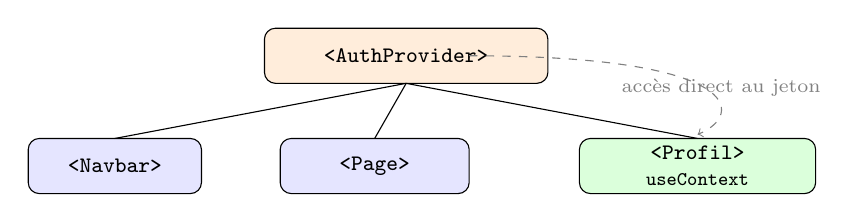
\begin{tikzpicture}[font=\footnotesize]
	\draw[fill=orange!14, rounded corners] (3.4,3.0) rectangle (7.0,3.7) node[midway]{\texttt{<AuthProvider>}};
	\draw[fill=blue!10, rounded corners] (0.4,1.6) rectangle (2.6,2.3) node[midway]{\texttt{<Navbar>}};
	\draw[fill=blue!10, rounded corners] (3.6,1.6) rectangle (6.0,2.3) node[midway]{\texttt{<Page>}};
	\draw[fill=green!14, rounded corners] (7.4,1.6) rectangle (10.4,2.3) node[midway, align=center]{\texttt{<Profil>}\\\scriptsize \texttt{useContext}};
	\draw (5.2,3.0) -- (1.5,2.3); \draw (5.2,3.0) -- (4.8,2.3); \draw (5.2,3.0) -- (8.9,2.3);
	\draw[->, dashed, gray] (6.0,3.35) .. controls (9.5,3.35) and (9.5,2.6) .. (8.9,2.35);
	\node[gray] at (9.2,2.95){\scriptsize accès direct au jeton};
\end{tikzpicture}
\end{center}
\noindent\textit{Figure~: le contexte rend le JWT disponible à tout l'arbre sans \og{}prop drilling\fg{}.} C'est la \textbf{piste de solution} retenue (combinée aux hooks) pour exposer proprement le jeton aux composants qui en ont besoin.

\newpage

\subsubsection*{Provider}
\phantomsection
\addcontentsline{toc}{subsection}{Provider}

\noindent Un \textbf{Provider} (\og{}fournisseur\fg{}) est le composant, livré par chaque contexte (\texttt{Contexte.Provider}), qui \textbf{englobe une portion de l'arbre} de composants et lui \textbf{fournit une valeur}. Tout composant placé \textbf{à l'intérieur} du Provider peut lire cette valeur, quel que soit son niveau de profondeur. Dans le projet, un \textbf{AuthProvider} centralise l'\textbf{état d'authentification} (le JWT, l'utilisateur courant et les fonctions \texttt{login}/\texttt{logout}) et l'expose à toute l'application~:
\begin{minted}[fontsize=\footnotesize, bgcolor=gray!8]{jsx}
import { createContext, useState } from 'react';

export const AuthContext = createContext(null);   // création du contexte

// Provider : englobe l'app et fournit le jeton + les actions
export function AuthProvider({ children }) {
  const [token, setToken] = useState(null);       // état partagé (le JWT)

  const login  = (jwt) => setToken(jwt);          // stocke le jeton
  const logout = ()    => setToken(null);         // efface le jeton

  return (
    <AuthContext.Provider value={{ token, login, logout }}>
      {children}
    </AuthContext.Provider>
  );
}
\end{minted}
\noindent On enveloppe alors l'application (\texttt{<AuthProvider><App/></AuthProvider>}) pour que tous les composants accèdent au jeton. Le Provider est le pivot de l'\textbf{access store} décrit ci-dessous.

\vspace{0.4cm}

\subsubsection*{Access store}
\phantomsection
\addcontentsline{toc}{subsection}{Access store}

\noindent Un \textbf{access store} (\og{}magasin d'accès\fg{}) est l'\textbf{état centralisé} qui détient les informations d'\textbf{authentification et d'accès} de l'utilisateur — au premier rang desquelles le \textbf{jeton JWT} — et les met à disposition de toute l'application de façon \textbf{contrôlée}. Plutôt que de disperser le jeton dans plusieurs composants, on le \textbf{regroupe en un point unique} (ici un contexte React via l'\texttt{AuthProvider}, ou une bibliothèque dédiée comme Redux/Zustand). Le store expose typiquement~:
\begin{itemize}
	\item la \textbf{valeur du jeton} et l'utilisateur courant (\textbf{source de vérité unique})~;
	\item les \textbf{actions} \texttt{login} / \texttt{logout} qui le mettent à jour~;
	\item un indicateur \textbf{\og{}est authentifié~?\fg{}} dérivé du jeton.
\end{itemize}
\noindent C'est la réponse directe à l'AAV \og{}Employer un access store\fg{}~: centraliser le jeton facilite sa \textbf{sécurisation} (un seul endroit à protéger), son \textbf{rafraîchissement} et son \textbf{effacement} à la déconnexion, ce qui répond à la problématique \og{}comment sécuriser son token côté frontend~?\fg{}.

\newpage

\subsubsection*{Hooks}
\phantomsection
\addcontentsline{toc}{subsection}{Hooks}

\noindent Les \textbf{hooks} sont des \textbf{fonctions spéciales} de React (préfixées par \texttt{use}) qui permettent à un \textbf{composant fonctionnel} de \og{}se brancher\fg{} sur des fonctionnalités avancées~: \textbf{état local}, \textbf{cycle de vie}, \textbf{contexte}, etc. Ils répondent à l'AAV \og{}Interagir avec les composants (hooks)\fg{}. Les principaux~:
\begin{itemize}
	\item \texttt{useState}~: ajoute un \textbf{état local} au composant (ex.~le chargement)~;
	\item \texttt{useEffect}~: exécute des \textbf{effets de bord} (appels API) selon le cycle de vie~;
	\item \texttt{useContext}~: \textbf{consomme un contexte} — ici, lire le \textbf{JWT} fourni par l'\texttt{AuthProvider}~;
	\item \textbf{hook personnalisé} (\texttt{useAuth})~: encapsule une logique réutilisable.
\end{itemize}
\noindent On crée souvent un \textbf{hook personnalisé} \texttt{useAuth} qui masque les détails du contexte et offre une \textbf{interface simple} aux composants~:
\begin{minted}[fontsize=\footnotesize, bgcolor=gray!8]{jsx}
import { useContext } from 'react';
import { AuthContext } from './AuthProvider';

// Hook personnalisé : accès simple et réutilisable au jeton
export function useAuth() {
  return useContext(AuthContext);                 // { token, login, logout }
}

// Dans un composant : on lit le JWT sans connaître le contexte
function BoutonDeconnexion() {
  const { logout } = useAuth();
  return <button onClick={logout}>Se déconnecter</button>;
}
\end{minted}
\noindent Combinés au \textbf{React Context}, les hooks constituent la \textbf{piste de solution} retenue pour exposer et manipuler le jeton de façon réutilisable dans tout le front-end.

\vspace{0.4cm}

\subsubsection*{Loadbalancing}
\phantomsection
\addcontentsline{toc}{subsection}{Loadbalancing}

\noindent Le \textbf{loadbalancing} (\textbf{répartition de charge}) consiste à \textbf{distribuer les requêtes entrantes} sur \textbf{plusieurs instances} d'un même service afin d'\textbf{absorber la charge}, d'\textbf{améliorer la disponibilité} (si une instance tombe, les autres prennent le relais) et d'assurer le \textbf{routage} vers le bon service. Un \textbf{répartiteur de charge} (\textit{load balancer}, ex.~\textbf{Nginx}) se place en \textbf{point d'entrée} et oriente chaque requête selon une stratégie (\textit{round-robin}, moindre charge…).
\begin{center}
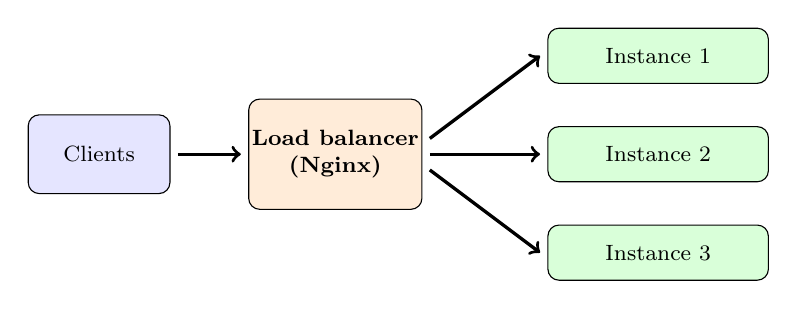
\begin{tikzpicture}[font=\footnotesize]
	\draw[fill=blue!10, rounded corners] (0,1.0) rectangle (1.8,2.0) node[midway]{Clients};
	\draw[fill=orange!15, rounded corners] (2.8,0.8) rectangle (5.0,2.2) node[midway, align=center]{\textbf{Load balancer}\\\textbf{(Nginx)}};
	\draw[->, very thick] (1.9,1.5) -- (2.7,1.5);
	\draw[fill=green!15, rounded corners] (6.6,2.4) rectangle (9.4,3.1) node[midway]{Instance 1};
	\draw[fill=green!15, rounded corners] (6.6,1.15) rectangle (9.4,1.85) node[midway]{Instance 2};
	\draw[fill=green!15, rounded corners] (6.6,-0.1) rectangle (9.4,0.6) node[midway]{Instance 3};
	\draw[->, very thick] (5.1,1.7) -- (6.5,2.75);
	\draw[->, very thick] (5.1,1.5) -- (6.5,1.5);
	\draw[->, very thick] (5.1,1.3) -- (6.5,0.25);
\end{tikzpicture}
\end{center}
\noindent\textit{Figure~: le répartiteur distribue les requêtes sur plusieurs instances et route vers le bon service.} C'est la réponse à l'AAV \og{}Utiliser le système de loadbalancing pour réaliser le routage\fg{}~: au-delà de la performance, le même \textbf{Nginx} sert de \textbf{point d'entrée} qui route les appels (et peut valider le \textbf{JWT}) vers les services en aval.

\newpage

\section*{Analyse et résolution : Sécurité}
\addcontentsline{toc}{section}{Analyse et résolution : Sécurité}

\noindent \textit{Rappel de la problématique~:} \og{}Comment sécuriser son token côté frontend~?\fg{}

\vspace{0.3cm}

\noindent Le back-end de Yanis délivre déjà des \textbf{JWT}~; le risque s'est donc déplacé \textbf{côté navigateur}, où le jeton doit être \textbf{stocké}, \textbf{transporté} et \textbf{exposé aux composants} sans jamais être dérobé. La réponse se construit en cinq étapes~: \textbf{(1)} le choix du \textbf{lieu de stockage} du jeton (et les menaces \textbf{XSS} / \textbf{CSRF}), \textbf{(2)} sa \textbf{centralisation} dans un \textbf{access store} (React Context + Provider), \textbf{(3)} son \textbf{exposition} via des \textbf{hooks} et des \textbf{composants réutilisables}, \textbf{(4)} son \textbf{transport sécurisé} vers l'API (en-tête \texttt{Authorization} et \textbf{CORS}), et \textbf{(5)} le \textbf{routage} par \textbf{loadbalancing} en point d'entrée. Une synthèse argumentée clôt l'analyse.

\vspace{0.4cm}

\subsection*{1. Où et comment stocker le jeton~? (menaces XSS / CSRF)}
\phantomsection
\addcontentsline{toc}{subsection}{1. Stockage du jeton (XSS / CSRF)}
\noindent Sécuriser le jeton commence par choisir \textbf{où le conserver}. Trois options s'offrent au front-end, avec des compromis de sécurité distincts~:
\begin{center}
\setlength{\tabcolsep}{6pt}
\begin{tabular}{|l|l|l|}
\hline
\textbf{Emplacement} & \textbf{Exposé au XSS} & \textbf{Exposé au CSRF} \\ \hline
\texttt{localStorage} & \textbf{oui} (lisible en JS) & non \\ \hline
Cookie \texttt{httpOnly} & \textbf{non} (illisible en JS) & oui (à mitiger) \\ \hline
Mémoire (variable JS) & limité & non \\ \hline
\end{tabular}
\end{center}
\noindent Deux menaces structurent le choix~: le \textbf{XSS} (\textit{Cross-Site Scripting}), où un script injecté \textbf{lit le jeton}, et le \textbf{CSRF} (\textit{Cross-Site Request Forgery}), où une requête est \textbf{émise à l'insu} de l'utilisateur. La meilleure protection consiste à confier le jeton à un \textbf{cookie \texttt{httpOnly}} (inaccessible au JavaScript, donc immunisé contre le vol par XSS), complété par l'attribut \texttt{SameSite=Strict} et un jeton anti-CSRF pour neutraliser le CSRF. Lorsqu'un cookie n'est pas envisageable, on conserve le jeton \textbf{en mémoire} dans l'\textbf{access store} (perdu au rechargement, mais jamais persisté en clair), en \textbf{durcissant le front contre le XSS} (échappement systématique, \textbf{CSP}). On évite \texttt{localStorage} pour un jeton sensible, précisément parce qu'il est lisible par tout script.

\vspace{0.4cm}

\subsection*{2. Centraliser le jeton dans un access store}
\phantomsection
\addcontentsline{toc}{subsection}{2. Centraliser dans un access store}
\noindent Plutôt que de disperser le jeton, on le \textbf{centralise en un point unique} — un \textbf{access store} bâti sur \textbf{React Context} et exposé par un \textbf{Provider}. Ce store devient la \textbf{source de vérité} de l'authentification (jeton, utilisateur, actions \texttt{login}/\texttt{logout}) et n'écrit \textbf{jamais} le jeton en clair dans un emplacement vulnérable~:

\begin{minted}[fontsize=\footnotesize, bgcolor=gray!8]{jsx}
import { createContext, useState, useContext } from 'react';

const AuthContext = createContext(null);

// Access store : le JWT vit EN MÉMOIRE (pas dans localStorage)
export function AuthProvider({ children }) {
  const [token, setToken] = useState(null);       // source de vérité unique

  const login  = (jwt) => setToken(jwt);          // après /login back-end
  const logout = ()    => setToken(null);         // efface le jeton

  const value = { token, login, logout, estAuth: Boolean(token) };
  return <AuthContext.Provider value={value}>{children}</AuthContext.Provider>;
}

export const useAuth = () => useContext(AuthContext);   // accès réutilisable
\end{minted}
\noindent En enveloppant l'application (\texttt{<AuthProvider><App/></AuthProvider>}), \textbf{un seul endroit} détient le jeton~: il est plus simple à \textbf{protéger}, à \textbf{rafraîchir} et à \textbf{effacer} à la déconnexion. C'est la réponse à l'AAV \og{}Employer un access store\fg{}.

\newpage

\subsection*{3. Exposer le jeton~: hooks et composants réutilisables}
\phantomsection
\addcontentsline{toc}{subsection}{3. Hooks et composants réutilisables}
\noindent Le store est consommé via le \textbf{hook} \texttt{useAuth}, qui masque les détails du contexte et offre une \textbf{interface simple} aux composants (AAV \og{}Interagir avec les composants (hooks)\fg{}). On en dérive des \textbf{composants réutilisables} qui encapsulent la logique de sécurité une fois pour toutes — par exemple une \textbf{route protégée} (AAV \og{}Développer des composants réutilisables\fg{})~:

\begin{minted}[fontsize=\footnotesize, bgcolor=gray!8]{jsx}
import { Navigate } from 'react-router-dom';
import { useAuth } from './AuthProvider';

// Composant réutilisable : protège n'importe quelle page
export function RouteProtegee({ children }) {
  const { estAuth } = useAuth();                  // lit le store via le hook
  return estAuth ? children : <Navigate to="/login" replace />;
}

// Usage : <RouteProtegee><Profil /></RouteProtegee>
\end{minted}
\noindent Ce composant, \textbf{indépendant et réutilisable}, applique le même contrôle à toutes les pages sensibles. \textbf{Point de sécurité essentiel}~: ce garde-fou relève de l'\textbf{expérience utilisateur} (ne pas afficher de pages inutiles) et reste \textbf{contournable}~; la \textbf{protection réelle est toujours imposée côté back-end} par la validation du JWT.

\vspace{0.4cm}

\subsection*{4. Transporter le jeton vers l'API (Authorization + CORS)}
\phantomsection
\addcontentsline{toc}{subsection}{4. Transport du jeton et CORS}
\noindent Le jeton est \textbf{joint automatiquement} à chaque requête sortante par un \textbf{intercepteur Axios} qui le lit dans le store et le place dans l'en-tête \texttt{Authorization: Bearer <token>}~:

\begin{minted}[fontsize=\footnotesize, bgcolor=gray!8]{jsx}
// Intercepteur : ajoute le JWT du store à chaque requête
api.interceptors.request.use((config) => {
  const { token } = store.getState().auth;        // jeton centralisé
  if (token) config.headers.Authorization = `Bearer ${token}`;
  return config;
});
\end{minted}
\noindent Comme le front (ex.~\texttt{app.breezy.fr}) et l'API (ex.~\texttt{api.breezy.fr}) sont sur des \textbf{origines différentes}, le navigateur applique la \textbf{politique du même origine} et \textbf{bloquerait} l'appel sans une \textbf{configuration CORS} explicite côté serveur. Le back-end doit donc \textbf{autoriser l'origine du front} et l'en-tête \texttt{Authorization}~:

\begin{minted}[fontsize=\footnotesize, bgcolor=gray!8]{javascript}
// Configuration CORS côté API (Express)
app.use(cors({
  origin: 'https://app.breezy.fr',       // seule origine autorisée
  methods: ['GET', 'POST', 'PUT', 'DELETE'],
  allowedHeaders: ['Authorization', 'Content-Type'],
  credentials: true,                     // si cookies httpOnly
}));
\end{minted}
\noindent On évite ainsi le \texttt{*} permissif~: \textbf{seule l'origine du front} est acceptée, ce qui répond à la contrainte \textbf{CORS} du projet tout en laissant passer le \textbf{JWT}.

\newpage

\subsection*{5. Routage par loadbalancing en point d'entrée}
\phantomsection
\addcontentsline{toc}{subsection}{5. Routage par loadbalancing}
\noindent En amont des services, un \textbf{répartiteur de charge Nginx} sert de \textbf{point d'entrée unique}~: il \textbf{route} les requêtes vers les bonnes instances, répartit la charge et peut \textbf{valider le JWT} avant de transmettre. Le front ne connaît ainsi qu'une seule adresse, et la sécurité est appliquée \textbf{au plus tôt}~:

\begin{minted}[fontsize=\footnotesize, bgcolor=gray!8]{nginx}
upstream api_backend {            # plusieurs instances -> répartition
  server api1:4000;
  server api2:4000;
}
server {
  listen 80;
  location /api/ {
    proxy_pass http://api_backend;          # routage + load balancing
    proxy_set_header Authorization $http_authorization;  # transmet le JWT
  }
}
\end{minted}
\noindent C'est la réponse à l'AAV \og{}Utiliser le système de loadbalancing pour réaliser le routage\fg{}~: un même point d'entrée assure \textbf{routage}, \textbf{disponibilité} et transmission contrôlée du jeton.

\vspace{0.4cm}

\subsection*{6. Architecture retenue (schéma argumenté)}
\phantomsection
\addcontentsline{toc}{subsection}{6. Architecture retenue}
\noindent L'utilisateur s'authentifie, reçoit un \textbf{JWT} qui est \textbf{centralisé dans l'access store}~; les \textbf{composants} le consomment via le \textbf{hook} \texttt{useAuth}, l'\textbf{intercepteur} le joint à chaque appel, et le \textbf{load balancer Nginx} route la requête vers l'API après franchissement du \textbf{CORS}.
\begin{center}
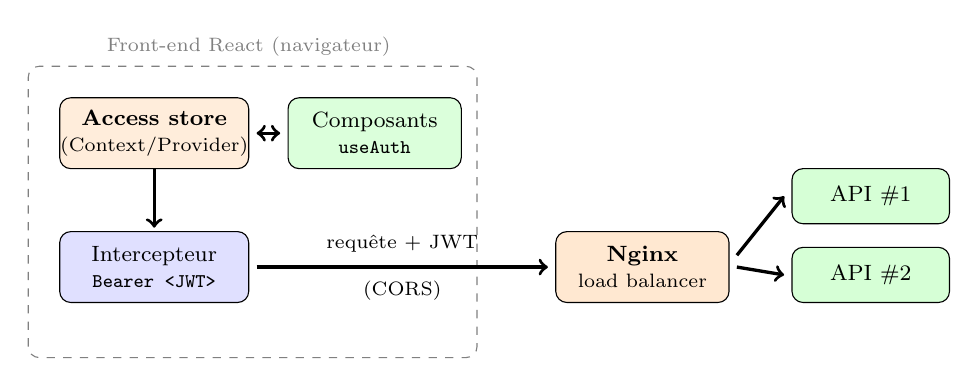
\begin{tikzpicture}[font=\footnotesize]
	\draw[dashed, gray, rounded corners] (-0.3,-0.3) rectangle (5.4,3.4);
	\node[gray] at (2.5,3.65){\scriptsize Front-end React (navigateur)};
	\draw[fill=orange!14, rounded corners] (0.1,2.1) rectangle (2.5,3.0) node[midway, align=center]{\textbf{Access store}\\\scriptsize (Context/Provider)};
	\draw[fill=green!14, rounded corners] (3.0,2.1) rectangle (5.2,3.0) node[midway, align=center]{Composants\\\scriptsize \texttt{useAuth}};
	\draw[fill=blue!12, rounded corners] (0.1,0.4) rectangle (2.5,1.3) node[midway, align=center]{Intercepteur\\\scriptsize \texttt{Bearer <JWT>}};
	\draw[<->, very thick] (2.6,2.55) -- (2.9,2.55);
	\draw[->, very thick] (1.3,2.1) -- (1.3,1.35);
	% load balancer
	\draw[fill=orange!18, rounded corners] (6.4,0.4) rectangle (8.6,1.3) node[midway, align=center]{\textbf{Nginx}\\\scriptsize load balancer};
	\draw[->, very thick] (2.6,0.85) -- (6.3,0.85); \node at (4.45,1.15){\scriptsize requête + JWT};
	\node at (4.45,0.55){\scriptsize (CORS)};
	% API
	\draw[fill=green!16, rounded corners] (9.4,1.4) rectangle (11.4,2.1) node[midway]{API \#1};
	\draw[fill=green!16, rounded corners] (9.4,0.4) rectangle (11.4,1.1) node[midway]{API \#2};
	\draw[->, very thick] (8.7,1.0) -- (9.3,1.75);
	\draw[->, very thick] (8.7,0.85) -- (9.3,0.75);
\end{tikzpicture}
\end{center}
\noindent\textit{Figure~: architecture retenue — jeton centralisé dans l'access store, consommé par les composants via hooks, transporté en \texttt{Bearer} à travers le CORS et routé par le load balancer Nginx.}

\vspace{0.2cm}

\noindent \textbf{Justification}~: chaque exigence est satisfaite — \textbf{jeton non exposé} (mémoire / cookie \texttt{httpOnly}, jamais \texttt{localStorage}), \textbf{centralisation} dans un access store unique, \textbf{exposition réutilisable} par hooks et composants, \textbf{transport contrôlé} via \texttt{Authorization} et une \textbf{CORS} restrictive, et \textbf{routage} par load balancer en point d'entrée.

\newpage

\subsection*{Conclusion}
\phantomsection
\addcontentsline{toc}{subsection}{Conclusion}
\noindent \textbf{En réponse à la problématique}, sécuriser le jeton côté front-end ne tient pas à une mesure unique mais à une \textbf{chaîne de décisions cohérentes}. Le premier choix est celui du \textbf{stockage}~: on écarte \texttt{localStorage} (lisible par un XSS) au profit d'un \textbf{cookie \texttt{httpOnly}} ou, à défaut, d'une conservation \textbf{en mémoire} dans l'access store, en durcissant le front contre le \textbf{XSS} et le \textbf{CSRF}.

\vspace{0.2cm}

\noindent Le jeton est ensuite \textbf{centralisé} dans un \textbf{access store} (React Context + Provider), \textbf{source de vérité unique} bien plus simple à protéger, rafraîchir et effacer. Il est \textbf{exposé} aux composants par le \textbf{hook} \texttt{useAuth} et par des \textbf{composants réutilisables} (route protégée), étant entendu que ce contrôle front relève de l'\textbf{UX}~: la \textbf{protection réelle reste imposée côté back-end}.

\vspace{0.2cm}

\noindent Enfin, le jeton est \textbf{transporté} en \texttt{Authorization: Bearer} via un intercepteur, à travers une \textbf{CORS restrictive} (seule l'origine du front autorisée), puis \textbf{routé} par un \textbf{load balancer Nginx} en point d'entrée unique. L'ensemble constitue un \textbf{modèle reproductible} de sécurisation du jeton côté client, applicable à toutes les interfaces de l'entreprise.

\newpage

\section*{Capitalisation}
\addcontentsline{toc}{section}{Capitalisation}

\begin{center}
\setlength{\tabcolsep}{10pt}

\begin{tabular}{|p{0.30\textwidth}|p{0.45\textwidth}|m{0.08\textwidth}|}
\hline
\textbf{AAV} & \textbf{Commentaire} & \textbf{Statut} \\ \hline

Développer des composants réutilisables &
Composant \texttt{RouteProtegee} indépendant et réutilisable, encapsulant le contrôle d'accès front et applicable à toute page sensible. &
{\color{green!60!black}Acquis} \\ \hline

Employer un access store &
Jeton centralisé dans un access store (React Context + Provider) servant de source de vérité unique (\texttt{token}, \texttt{login}, \texttt{logout}), illustré par du code commenté. &
{\color{green!60!black}Acquis} \\ \hline

Interagir avec les composants (hooks) &
Hooks React (\texttt{useState}, \texttt{useContext}) et hook personnalisé \texttt{useAuth} exposant le jeton aux composants de façon simple et réutilisable. &
{\color{green!60!black}Acquis} \\ \hline

Utiliser (Modéliser) JWT pour le processus d'authentification &
Processus modélisé~: jeton délivré au \texttt{login}, stocké sans exposition (cookie \texttt{httpOnly}/mémoire vs \texttt{localStorage}), joint en \texttt{Bearer} et validé côté back-end. &
{\color{green!60!black}Acquis} \\ \hline

Utiliser le système de loadbalancing pour réaliser le routage &
Load balancer Nginx en point d'entrée unique répartissant la charge sur plusieurs instances et routant les requêtes (avec transmission du JWT), illustré par une configuration. &
{\color{green!60!black}Acquis} \\ \hline

\end{tabular}
\end{center}

\newpage

\section*{Ressources}
\addcontentsline{toc}{section}{Ressources}

\begin{itemize}
	\item \textbf{JWT (introduction \& débogueur)} : \url{https://jwt.io/introduction}
	\item \textbf{MDN -- CORS (Cross-Origin Resource Sharing)} : \url{https://developer.mozilla.org/fr/docs/Web/HTTP/CORS}
	\item \textbf{React -- Context} : \url{https://react.dev/learn/passing-data-deeply-with-context}
	\item \textbf{React -- Hooks (useContext)} : \url{https://react.dev/reference/react/useContext}
	\item \textbf{OWASP -- JWT \& stockage côté client (Cheat Sheet)} : \url{https://cheatsheetseries.owasp.org/cheatsheets/JSON_Web_Token_for_Java_Cheat_Sheet.html}
	\item \textbf{OWASP -- Cross-Site Scripting (XSS)} : \url{https://owasp.org/www-community/attacks/xss/}
	\item \textbf{OWASP -- Cross-Site Request Forgery (CSRF)} : \url{https://owasp.org/www-community/attacks/csrf}
	\item \textbf{Documentation Axios (intercepteurs)} : \url{https://axios-http.com/fr/docs/interceptors}
	\item \textbf{Nginx -- répartition de charge (load balancing)} : \url{https://docs.nginx.com/nginx/admin-guide/load-balancer/http-load-balancer/}
\end{itemize}
